\subsubsection{Casos Patologicos}
Caso particular chiquito, página 3. Fijate el parrafo que arranca en A simple apprroach...... y despues This approach ignores that... La idea es armar el mismo grafo y mostrar el mismo ejemplo jaja

\begin{figure}[H]
\centering
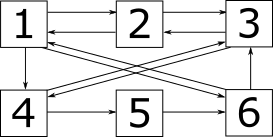
\includegraphics[scale=1.0]{images/grafo.png}
\caption{Caso de estudio}
\label{casoEst}
\end{figure}

\begin{table}[H]
\centering
\caption{My caption}
\label{my-label}
\begin{tabular}{lll}
\hline
Nro. Web & PageRank & Por grado \\ \hline
1        & 0.164204 & 3         \\
2        & 0.172456 & 2         \\
3        & 0.237500 & 2         \\
4        & 0.172456 & 2         \\
5        & 0.098296 & 1         \\
6        & 0.155089 & 2         \\ \hline
\end{tabular}
\end{table}